\documentclass[12pt]{beamer}
\usepackage[utf8]{inputenc}
\usetheme{default}
\usepackage{pgf,pgfarrows,pgfnodes}
\usepackage{graphicx}
\usepackage{algorithmicx} 
\usepackage{color}
\usepackage{lipsum}  
\usepackage{xcolor}
\usepackage{pdfpages}
\usepackage{hyperref}
\usepackage[english]{babel}
\usepackage{graphicx}
\usepackage{ragged2e}
\usepackage{tikz}
\usepackage{multirow}
\usepackage{tabularx}
\usepackage{array}
\usepackage{mathptmx}       % selects Times Roman as basic font
\usepackage{helvet}         % selects Helvetica as sans-serif font
\usepackage{courier}        % selects Courier as typewriter font
\usepackage{type1cm}        % activate if the above 3 fonts are
\usepackage{textpos} 
\usepackage{pgf,pgfarrows,pgfnodes}
\usepackage{graphicx}
\usepackage{color}
\usepackage{natbib}
\setbeamersize{text margin left=10pt,text margin right=10pt}
\definecolor{idrbt_dark_blue}{HTML}{3333b3}
\definecolor{idrbt_blue}{HTML}{00AEEF} 
\definecolor{adroit_black}{HTML}{222222}
\let\oldcite=\cite                                                              
\renewcommand{\cite}[1]{\textcolor[rgb]{0,.7,0}{\oldcite{#1}}}
\setbeamercolor{item}{fg=idrbt_blue}
\setbeamertemplate{section in toc}
{\leavevmode\leftskip=2ex%
	\llap{%
		\usebeamerfont*{section number projected}%
		\usebeamercolor{section number projected}%
		\begin{pgfpicture}{-1ex}{0ex}{1ex}{2ex}
			\color{idrbt_blue}
			%      \color{red}
			\pgfpathcircle{\pgfpoint{0pt}{.75ex}}{1.7ex}
			\pgfusepath{fill}
			\pgftext[base]{\color{fg}\inserttocsectionnumber}
		\end{pgfpicture}\kern1.25ex%
	}%
	\inserttocsection\par}
\date{}
\title{\textcolor{idrbt_blue}{\rule{112mm}{1.25mm}} \textbf{Lecture-4:\\ Introduction to R}
	 \textcolor{idrbt_blue}{\rule{112mm}{1.25mm}}}
\author{\textcolor{red}{\texttt{\textbf{Manu.V.T.}\\ 
			{\scriptsize Senior Research Fellow\\ Center of Excellence in Cyber Security\\IDRBT}}} }%\newline {\scriptsize Research Fellow} }
%%%%%%%%%%%%%%%%%%%%%%%%%%%%%%%%%%%%%%%%%%%%%%%%%%%%%%%%%%%%%%
\makeatletter
\long\def\beamer@section[#1]#2{%
	\beamer@savemode%
	\mode<all>%
	\ifbeamer@inlecture
	\refstepcounter{section}%
	\beamer@ifempty{#2}%
	{\long\def\secname{#1}\long\def\lastsection{#1}}%
	{\global\advance\beamer@tocsectionnumber by 1\relax%
		\long\def\secname{#2}%
		\long\def\lastsection{#1}%
		\addtocontents{toc}{\protect\beamer@sectionintoc{\the\c@section}{#2\hfill\the\c@page}{\the\c@page}{\the\c@part}%
			{\the\beamer@tocsectionnumber}}}%
	{\let\\=\relax\xdef\sectionlink{{Navigation\the\c@page}{\noexpand\secname}}}%
	\beamer@tempcount=\c@page\advance\beamer@tempcount by -1%
	\beamer@ifempty{#1}{}{%
		\addtocontents{nav}{\protect\headcommand{\protect\sectionentry{\the\c@section}{#1}{\the\c@page}{\secname}{\the\c@part}}}%
		\addtocontents{nav}{\protect\headcommand{\protect\beamer@sectionpages{\the\beamer@sectionstartpage}{\the\beamer@tempcount}}}%
		\addtocontents{nav}{\protect\headcommand{\protect\beamer@subsectionpages{\the\beamer@subsectionstartpage}{\the\beamer@tempcount}}}%
	}%
	\beamer@sectionstartpage=\c@page%
	\beamer@subsectionstartpage=\c@page%
	\def\insertsection{\expandafter\hyperlink\sectionlink}%
	\def\insertsubsection{}%
	\def\insertsubsubsection{}%
	\def\insertsectionhead{\hyperlink{Navigation\the\c@page}{#1}}%
	\def\insertsubsectionhead{}%
	\def\insertsubsubsectionhead{}%
	\def\lastsubsection{}%
	\Hy@writebookmark{\the\c@section}{\secname}{Outline\the\c@part.\the\c@section}{2}{toc}%
	\hyper@anchorstart{Outline\the\c@part.\the\c@section}\hyper@anchorend%
	\beamer@ifempty{#2}{\beamer@atbeginsections}{\beamer@atbeginsection}%
	\fi%
	\beamer@resumemode}%

\def\beamer@subsection[#1]#2{%
	\beamer@savemode%
	\mode<all>%
	\ifbeamer@inlecture%
	\refstepcounter{subsection}%
	\beamer@ifempty{#2}{\long\def\subsecname{#1}\long\def\lastsubsection{#1}}
	{%
		\long\def\subsecname{#2}%
		\long\def\lastsubsection{#1}%
		\addtocontents{toc}{\protect\beamer@subsectionintoc{\the\c@section}{\the\c@subsection}{#2\hfill\the\c@page}{\the\c@page}{\the\c@part}{\the\beamer@tocsectionnumber}}%
	}%
	\beamer@tempcount=\c@page\advance\beamer@tempcount by -1%
	\addtocontents{nav}{%
		\protect\headcommand{\protect\beamer@subsectionentry{\the\c@part}{\the\c@section}{\the\c@subsection}{\the\c@page}{\lastsubsection}}%
		\protect\headcommand{\protect\beamer@subsectionpages{\the\beamer@subsectionstartpage}{\the\beamer@tempcount}}%
	}%
	\beamer@subsectionstartpage=\c@page%
	\edef\subsectionlink{{Navigation\the\c@page}{\noexpand\subsecname}}%
	\def\insertsubsection{\expandafter\hyperlink\subsectionlink}%
	\def\insertsubsubsection{}%
	\def\insertsubsectionhead{\hyperlink{Navigation\the\c@page}{#1}}%
	\def\insertsubsubsectionhead{}%
	\Hy@writebookmark{\the\c@subsection}{#2}{Outline\the\c@part.\the\c@section.\the\c@subsection.\the\c@page}{3}{toc}%
	\hyper@anchorstart{Outline\the\c@part.\the\c@section.\the\c@subsection.\the\c@page}\hyper@anchorend%
	\beamer@ifempty{#2}{\beamer@atbeginsubsections}{\beamer@atbeginsubsection}%
	\fi%
	\beamer@resumemode}

\makeatother
%%%%%%%%%%%%%%%%%%%%%%%%%%%%%%%%%%%%%%%%%%%%%%%%%%%%%%%%%%%%%%
\beamertemplatenavigationsymbolsempty

\addtobeamertemplate{navigation symbols}{}{%
	\usebeamerfont{footline}%
	\usebeamercolor[fg]{footline}%
	\hspace{1em}%
	\insertframenumber/\inserttotalframenumber
}
%%%%%%%%%%%%%%%%%%%%%%%%%%%%%%%%%%%%%%%%%%%%%%%%%%%%%%%%%%%%%%
\begin{document}
	%%%%%%%%%%%%%%%%%%%%%%%%%%%%%%%%%%%%%%%%%%%%%%%%%%%%%%%%%%%%%%%%%%%%%%%%%%%%%%%%%%%%%%%%%%%%%%%%%%%%%%%%%%%%%%%%%%%%%%%%%%%%%
	
	\begin{frame}
	\titlepage
	


\begin{center}
			\begin{tabular}{l>{\centering}p{6.25cm}<{\centering}l}
			\multirow{1}{*}{
\includegraphics[scale=0.15]{./IDRBT_lowres.png}}
			&
         
			&
			\multirow{1}{*}{
\includegraphics[scale=0.2]{./uoh.png}}
		\end{tabular}
\end{center}

\smallskip
	\renewcommand*{\arraystretch}{1.05}



\end{frame}
%%%%%%%%%%%%%%%%%%%%%%%%%%%%%%%%%%%%%%%%%%%%%%%%%%%%%%%%%%%%%%%%%%%%%%%%%%%%%%%%%%%%%%%%%%%%%%%%%%%%%%%%%%%%%%%%%%%%%%%%%%%%%

\begin{frame}
\frametitle{Outline}
\tableofcontents %[hideallsubsections]
\end{frame}
%%%%%%%%%%%%%%%%%%%%%%%%%%%%%%%%%%%%%%%%%%%%%%%%%%%%%%%%%%%%%%%%%%%%%%%%%%%%%%%%%%%%%%%%%%%%%%%%%%%%%%%%%%%%%%%%%%%%%%%%%%%%%

%%%%%%%%%%%%%%%%%%%%%%%%%%%%%%%%%%%%%%%%%%%%%%%%%%%%%%%%%%%%%%%%%%%%%%%%%%%%%%%%%%%%%%%%%%%%%%%%%%%%%%%%%%%%%%%%%%%%%%%%%%%%%
\begin{frame}
\section{Introduction}
\frametitle{Introduction }
	\begin{itemize}\justifying
		\item R is an open source programming language and software environment for statistical computing and graphics that is supported by the R Foundation for Statistical Computing
	  		\item R is a GNU package.
	  		\item The source code for the R software environment is written primarily in C, Fortran, and R.
			\item R has a command line interface, there are several graphical front-ends available.
	\end{itemize}
\end{frame}
%%%%%%%%%%%%%%%%%%%%%%%%%%%%%%%%%%%%%%%%%%%%%%%%%%%%%%%%%%%%%%%%%%%%%%%%%%%%%%%%%%%%%%%%%%%%%%%%%%%%%%%%%%%%%%%%%%%%%%%%%%%%%
\begin{frame}
\section{How to Use R?}
\frametitle{How to Use R?}
\begin{itemize}\justifying
	\item R installation directory
	\begin{itemize}
		\item R.home()
	\end{itemize}
	\item Check your working path
	\begin{itemize}
		\item getwd()
	\end{itemize}
	\item Change your working path
		\begin{itemize}
		\item setwd()
	\end{itemize}
	\item Use hash \# to comment
\end{itemize}
\end{frame}
%%%%%%%%%%%%%%%%%%%%%%%%%%%%%%%%%%%%%%%%%%%%%%%%%%%%%%%%%%%%%%%%%%%%%%%%%%%%%%%%%%%%%%%%%%%%%%%%%%%%%%%%%%%%%%%%%%%%%%%%%%%%%

\begin{frame}
\frametitle{Use R as Calculator}
\begin{tabular}{ll}
 Addition &+\\
 Subtraction &-\\
 Multiplication &*\\
 Division &/\\
 Exponent &\^{} OR **\\
 Modulus &$(x$ mod $y)$ OR $x$\%\%$y$\\
 Integer Division &$x$\%/\%$y$\\
\end{tabular}
\end{frame}

\begin{frame}
\frametitle{Operators used in R}
\begin{tabular}{ll}
$<$ &Less than\\
$<=$ &Less than or equal to\\
$>$ &Greater than\\
$>=$ &Greater than or equal to\\
$==$ &Exactly equal to (similar to =)\\
$!=$ &Not equal to\\
\end{tabular}
\end{frame}

\begin{frame}[fragile]
\section{Workspace in R}
\frametitle{Workspace in R }
\begin{itemize}\justifying
	\item Save Workspace
	\begin{itemize}\justifying
		\item save.image()\hfill \# Default file .Rdata
		\item unlink(“.RData”) \hfill \# To remove
		\item save.image(“mywork.Rdata”)\hfill  \# In specific file
		\item load(“mywork.Rdata”)\hfill  \# Load previous work
		\item savehistory(file=”abc”)\hfill  \# Save in txt file, default .Rhistory
		\item loadhistory(file=”abc”) \hfill \# Load history from file
	\end{itemize}
	\item Quit Session
	\begin{itemize}\justifying
	\item q() \hfill \# It will ask to save the workspace image?\hfill  \verb|[y/n/c]|
\end{itemize}
\end{itemize}
\end{frame}

\begin{frame}[fragile]
\frametitle{Getting help in R }
\begin{itemize}\justifying
	\item Within R:
	\begin{itemize}\justifying
		\item $?$ keyword or help(keyword)  \hfill \# Command search
		\item library(help=pamr)
		\item $??$keyword or help.search(“keyword”)  \hfill \# If don’t know function
		\item apropos("mean")  \hfill \# list all functions containing
		string mean
	\end{itemize}
	\item Documentation
	\begin{itemize}\justifying
		\item Help files can be accessed in the text file or html format.
		\item Manuals, reference cards, tutorials and news about recent developments
		are available at \\ \verb|http://www.r-project.org/other-docs.html|
	\end{itemize}
\end{itemize}
\end{frame}

\begin{frame}[fragile]
\section{Data Types in R }
\frametitle{Data Types in R }
\begin{itemize}\justifying
	\item Within R:
	\begin{itemize}\justifying
		\item $?$ keyword or help(keyword)  \hfill \# Command search
		\item library(help=pamr)
		\item $??$keyword or help.search(“keyword”)  \hfill \# If don’t know function
		\item apropos("mean")  \hfill \# list all functions containing
		string mean
	\end{itemize}
	\item Documentation
	\begin{itemize}\justifying
		\item Help files can be accessed in the text file or html format.
		\item Manuals, reference cards, tutorials and news about recent developments
		are available at \\ \verb|http://www.r-project.org/other-docs.html|
	\end{itemize}
\end{itemize}
\end{frame}

\begin{frame}[fragile]
\frametitle{Variable types in R }
\begin{itemize}\justifying
	\item \textcolor{red}{Numeric}
	\begin{itemize}\justifying
		\item \textcolor{red}{Integer} \\
		$x = 6$\\
		is.real(x) \hfill \# TRUE\\
		is.integer(x)  \hfill \# FALSE\\
	\end{itemize}
	\item \textcolor{red}{Logical}\\
	$x = c(1,2,3,4,5); y = (x<3);$
	\item \textcolor{red}{Character String}\\
	x = c("M”)\\
	x = c("Kinjal","Madhav","Roopa","Suraj")\\
	\item \textcolor{red}{List} : collection of several objects of any type\\
	x1 = c("gene1","gene2","gene3","gene4",”gene5”)\\
	x2 = c(2,4,7,9,11)\\
	x = list(x1,x2)
	\item \textcolor{red}{Complex arithmetic}\\
	z = complex(real = rnorm(10), imag = rnorm(10))\\
	Re(z) \&	Im(z)\\
\end{itemize}
\end{frame}

\begin{frame}[fragile]
\frametitle{Vectors in R}
\begin{itemize}\justifying
	\item Vectors may have mode “logical”,”numeric”,”character”.
	\begin{itemize}\justifying
		\item Examples of Vectors\\
		x = c(45, 90, 135 )\\
		y = c("Kinjal","Madhav","Roopa","Suraj")\\
		z = c(" gene1 " , " gene2 " , " gene3 " , " gene4" )
	\end{itemize}
\end{itemize}
\end{frame}

\begin{frame}[fragile]
\frametitle{Arrays in R}
\begin{itemize}\justifying
	\item Vectors may also have mode “logical”,”numeric”,”character”.
	\item Two dimension array is same as matrix
	\item Examples of Two dimension array\\
	x = array(data, dim)\\
	x = array(1:3, c(2,4))\\
	\item Examples of Three dimension array\\
	x = array(1:3, c(2,4,2)) \hfill\# 2, represent the dimension\\
	x = array(1:3, c(2,4,3)) \hfill\# 3, represent the dimension\\
\end{itemize}
\end{frame}

\begin{frame}[fragile]
\frametitle{Matrices in R}
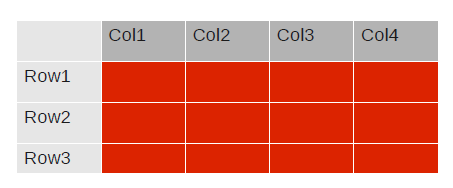
\includegraphics[scale=0.5]{Matrix}
\begin{itemize}\justifying
	\item Is a matrix
		\item Dimension : 3 $\times$ 4
		\item Row names : Row1, Row2, Row3
		\item Column names : Col1, Col2, Col3
		\item Row size: 3
		\item Column size: 4
\end{itemize}
\end{frame}

\begin{frame}[fragile]
\frametitle{Data frames in R}
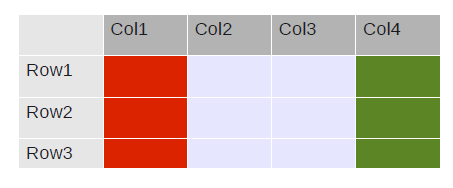
\includegraphics[scale=0.5]{DataFRame}
\begin{itemize}\justifying
	\item Data frame is a generalization of a matrix
	\item Different column may have different data types
	\item All elements of any column must ,have the same datatype, i.e.
	all numeric, or all factor, or all character, or all logical
		\item Use for R modeling and graphical functions
		\item If the data is read in using the command read.csv, read.txt etc, it will
	automatically be saved as a data frame.
\end{itemize}
\end{frame}

\begin{frame}[fragile]
\frametitle{Data Lists in R}
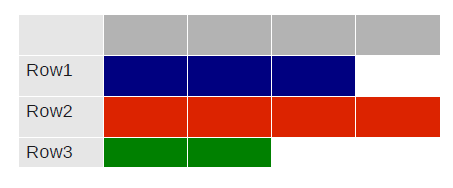
\includegraphics[scale=0.5]{DataLists}
\begin{itemize}\justifying
	\item Data list is arrangement of different lists
		\item Different rows may have different number of variables
		\item  All elements of any rows must ,have the same datatype, i.e.
	all numeric, or all factor, or all character, or all logical
\end{itemize}
\end{frame}

\begin{frame}[fragile]
\frametitle{Data Creation : Vectors and Arrays}
\begin{itemize}\justifying
	\item c(1,2,3,4) \hfill \# combine argument to create a vector
	\item  from:to  \hfill \# create sequence from to to
	\item seq(from,to,by=diff)  \hfill \# create airthmetic series
	\item  rep(c(1,2,3,4),4)  \hfill \# Replicate Elements of Vectors
	\item  array(1:3, c(2,4))  \hfill \# create array of size 2$\times$4
	\item  array(1:3, c(2,4,2))  \hfill \# create two array of size 2$\times$4
\end{itemize}
\end{frame}

\begin{frame}[fragile]
\frametitle{Data Creation : Arrays}
\begin{itemize}\justifying
	\item x = array(data, dim)
	\item x = array(1:3, c(2,4))
	\item x = array(1:3, c(2,4,2))   \hfill \# 2, represent the dimension
	\item x = array(1:3, c(2,4,3))   \hfill \# 3, represent the dimension
\end{itemize}
\end{frame}

\begin{frame}[fragile]
\frametitle{Data creation : Matrices in R}
a = 1:3\\
b = 4:6\\
c = 7:9
\begin{itemize}\justifying
	\item X = cbind(a,b,c) \hfill \# cbind combined object by Column
	\item Y = rbind(a,b,c) \hfill \# rbind combined object by Row
	\item Z = matrix(c(1,4,6,2,3,7.8), nrow=2, ncol=3, byrow=T) \\ \# Matrix by defining number of rows and columns
		\item  Z = matrix(c(1,4,6,2,3,7.8), nrow=2, ncol=3, byrow=F)
		\item  expression\_data = matrix(c(1,2,3, 11,12,13), nrow = 2, ncol=3,byrow=TRUE,dimnames =list(c("gene1", "gene2"),c("Sample.1","Sample.2", "Sample.3")))
		\item  replicate(5, rnorm(10)) \hfill \# To generate random matrix of 10 rows and 5 columns

\end{itemize}
\end{frame}



\begin{frame}[fragile]
\frametitle{Data Creation : Data frames}
\begin{itemize}\justifying
	\item go.term = c (“GO0009117”,”GO0009253”,”GO0009354”)
	\item  gene.count = c(15,18,25)
	\item 	 avg.expression.value = c(0.5432,0.2371,0.7867)
	\item  go.term.rank.rank= c(2,1,3)
	\item  mydata = data.frame
	(go.term,gene.count,avg.gene.expression,\\go.term.rank)
	\item  mydata2 =
	data.frame(\\rank=1:4,\\gene\_name= c("ddr1","apr2","bac","p53"),\\n=
	c(.90,.75,.52,.31));
\end{itemize}
\end{frame}



\begin{frame}[fragile]
\frametitle{Data Creation : Data Lists}
\begin{itemize}\justifying
	\item genelist1 = c (“abc1”,”abc2”)
	\item  genelist2 = c(“brca1”,”brca2”,”tp53”,”mdm2”)
	\item genelist3 = c(“apr”,”erpn”,”myc”)
	\item  mylist = list (genelist1,genelist2,genelist3)
	\item  mylist2 =
	list(rank=1:4,gene\_name=c("ddr1","apr2","bac","p53"),n=c(.90,.75,.52,.
	31));
\end{itemize}
\end{frame}
\begin{frame}
 \begin{center}
\begin{block}{}
\hspace*{2in}\textbf{\LARGE \textcolor{idrbt_dark_blue}{T}\pause
			    \textcolor{idrbt_blue}{h}\pause
			    \textcolor{idrbt_dark_blue}{a}\pause
			    \textcolor{idrbt_blue}{n}\pause
			    \textcolor{idrbt_dark_blue}{k}\pause
			    \textcolor{idrbt_dark_blue}{Y}\pause
			    \textcolor{idrbt_blue}{o}\pause
			    \textcolor{idrbt_dark_blue}{u} }
\end{block}\end{center}
\end{frame}
\end{document}
%%%%%%%%%%%%%%%%%%%%%%%%%%%%%%%%%%%%%%%%%%%%%%%%%%%%%%%%%%%%%%%%%%%%%%%%%%%%%%%%%%%%%%%%%%%%%%%%%%%%%%%%%%%%%%%%%%%%%%%%%%%%%